\documentclass{article}
\usepackage{graphicx}
\usepackage{subcaption}

% to make table of contents clickable
\usepackage{hyperref}
\hypersetup{
}

\author{CD}
\title{DD}

\begin{document}

\thispagestyle{empty} % to hide pagenum
\begin{center}

	\vspace{3cm}

	\large $\bf Software$ $\bf Engineering$ $\bf 2$

  
\includegraphics[width=\linewidth]{../RASD/images/polimi-logo.png}
  \vspace{2cm}
  

  \Huge $\bf SafeStreets$


	\huge $\bf Design$  $\bf Document$

	\vspace{1cm}

  Authors:
	\vspace{1cm}
	\begin{tabular}{r|l}
		 Federico Cazzola & \large mat 945835\\
		 Francesco Dotti & \large mat 945232\\
	\end{tabular}

	\vspace{1cm}

  Professor: Di Nitto Elisabetta
	
	\vspace{3cm}
  \normalsize Academic Year 2019-2020

	\vspace{2mm}
	\small Version 1.0

\end{center}

\newpage

\thispagestyle{empty} % to hide pagenum
\tableofcontents

\newpage
  
\section{Introduction}
\subsection{Purpose}
The purpose of this document is to describe how the system will be built, giving specific and technical details about architectural and design decisions. Also implementation, integration and testing plans will be discussed.
In particular the document presents:
\begin{itemize}
	\item The SafeStreet System architecture (its parts and how they interact)
	\item The runtime behavior
	\item The design patterns
	\item User Interfaces
	\item Implementation, integration and testing plans 
\end{itemize}

\subsection{Scope}
The scope of the Safestreets project, as already specified in the RASD, is to give the user the possibility to report traffic violation, in particular, parking violation (eg. parking in a spot reserved for disabled people, parking in an helicopter pitch, parking on the sidewalk).\\
The system will allow the users to select the type of violation leading to differt amount of ticket value.\\
The system will help the authorities to identify more infractions and therefore to issue more tickets which should increase the attention and respect of the citizens regarding the traffic rules.\\
Furthermore, thanks to the increased number of tickets, the municipality will have more money to invest in the community. This extra money could be used to do some interventions following the suggestions provided by SafeStreets.

\subsection{Definitions, Acronyms, Abbreviations}
\subsubsection{Definitions}
\begin{itemize}
\item \textbf{Mine}: to process data for obtaining new data
\item \textbf{Violation}: an infringement of the rules
\item \textbf{Unsafe}: area area where often happen violation and accident
\end{itemize}

\subsubsection{Acronyms}
\begin{itemize}
	\item \textbf{RASD}: Requirements Analysis and Specifications Document  
	\item \textbf{DD}: Design Document
	\item \textbf{FOSS}: Free and Open Source Software
	\item \textbf{S2B}: Software to Be
	\item \textbf{API}: Application Programming Interface
	\item \textbf{NIST}: National Institute of Standards and Technology
	\item \textbf{RFC}: Request for Comments
	\item \textbf{ALPR}: Automated License Plate Recognition
	\item \textbf{JWT}: JSON Web Tokens
\end{itemize}

\subsubsection{Abbreviations}
% \begin{itemize}
% \end{itemize}

\subsection{Revision history}
\begin{itemize}
	\item Version 1.0 | First Release
\end{itemize}

\subsection{Reference Documents}
\begin{itemize}
	\item Specification document: “SafeStreets Mandatory Project Assignment” 	
	\item \href{https://www.uml-diagrams.org}{UML diagrams}
	\item IEEE Standard for Information Technology—Systems Design—Software Design Descriptions (IEEE Std 1016TM-2009)
\end{itemize}

\subsection{Document Structure}
\begin{itemize}
	\item Chapter 1 is the introduction.
	\item Chapter 2 provides details about the system architecture, its components and how they interact.
	\item Chapter 3 describes the UX and shows the user interface providing mockups.
	\item Chapter 4 describes how the requirements ( defined in the RASD ) are mapped to the design elements defined in this document.
	\item Chapter 5 presents the implementation, integration and test plan. It shows how the different components of the application are integrated with each other and how they react. Also the testing strategies are described and the risks in the application are analyzed.
	\item Chapter 6 shows the effort spent by each group member
\end{itemize}

\newpage

\section{Architectural design}
\subsection{Overview: High-level components and their interaction}
The application will be developed with three logic software layers: 
\begin{itemize}
	\item Presentation (P) manages the user interaction with the system 
	\item Application (A) handles the business logic of the application and its functionalities 
	\item Data access (D) manages the information with access to the database
\end{itemize}
These layers are thought to be divided on three different hardware tiers (a machine or a group of machines), so that any logic layer has, in principle, its own dedicated hardware (three-tier architecture).\\
This architecture should give the system more scalability and flexibility as the server side is split into two nodes.\\
The second tier must contain only the business logic to physically separate clients and data to guarantee more safety in accessing to data since the system deals with sensitive data. \\
The following image shows an high-level view of the architecture of the system using the ArchiMate modeling language.\\
\\
\begin{figure}[ht]
\centering
	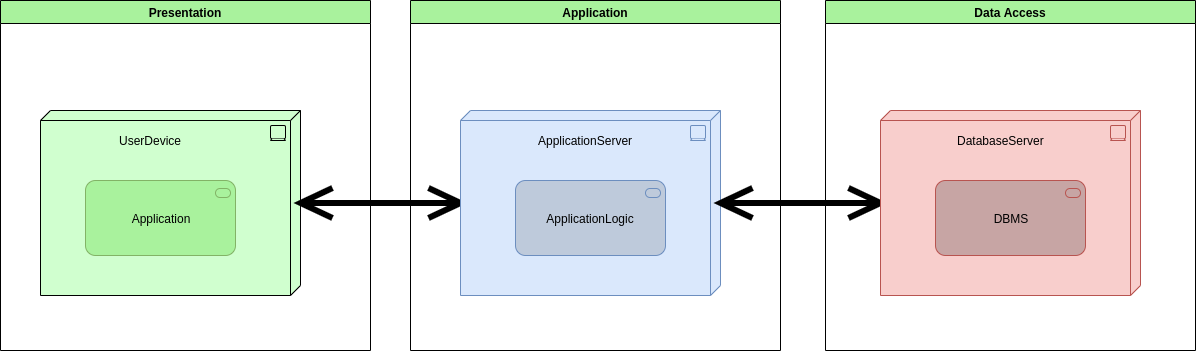
\includegraphics[width=1.0\textwidth]{images/tier-structure.png}
	\caption{SafeStreets 3-tier architecture}
	\label{fig:tier-structure}
\end{figure}

\newpage

\subsection{Component view}

In the following diagram only the application server is analyzed in detail

\begin{figure}[ht]
\centering
	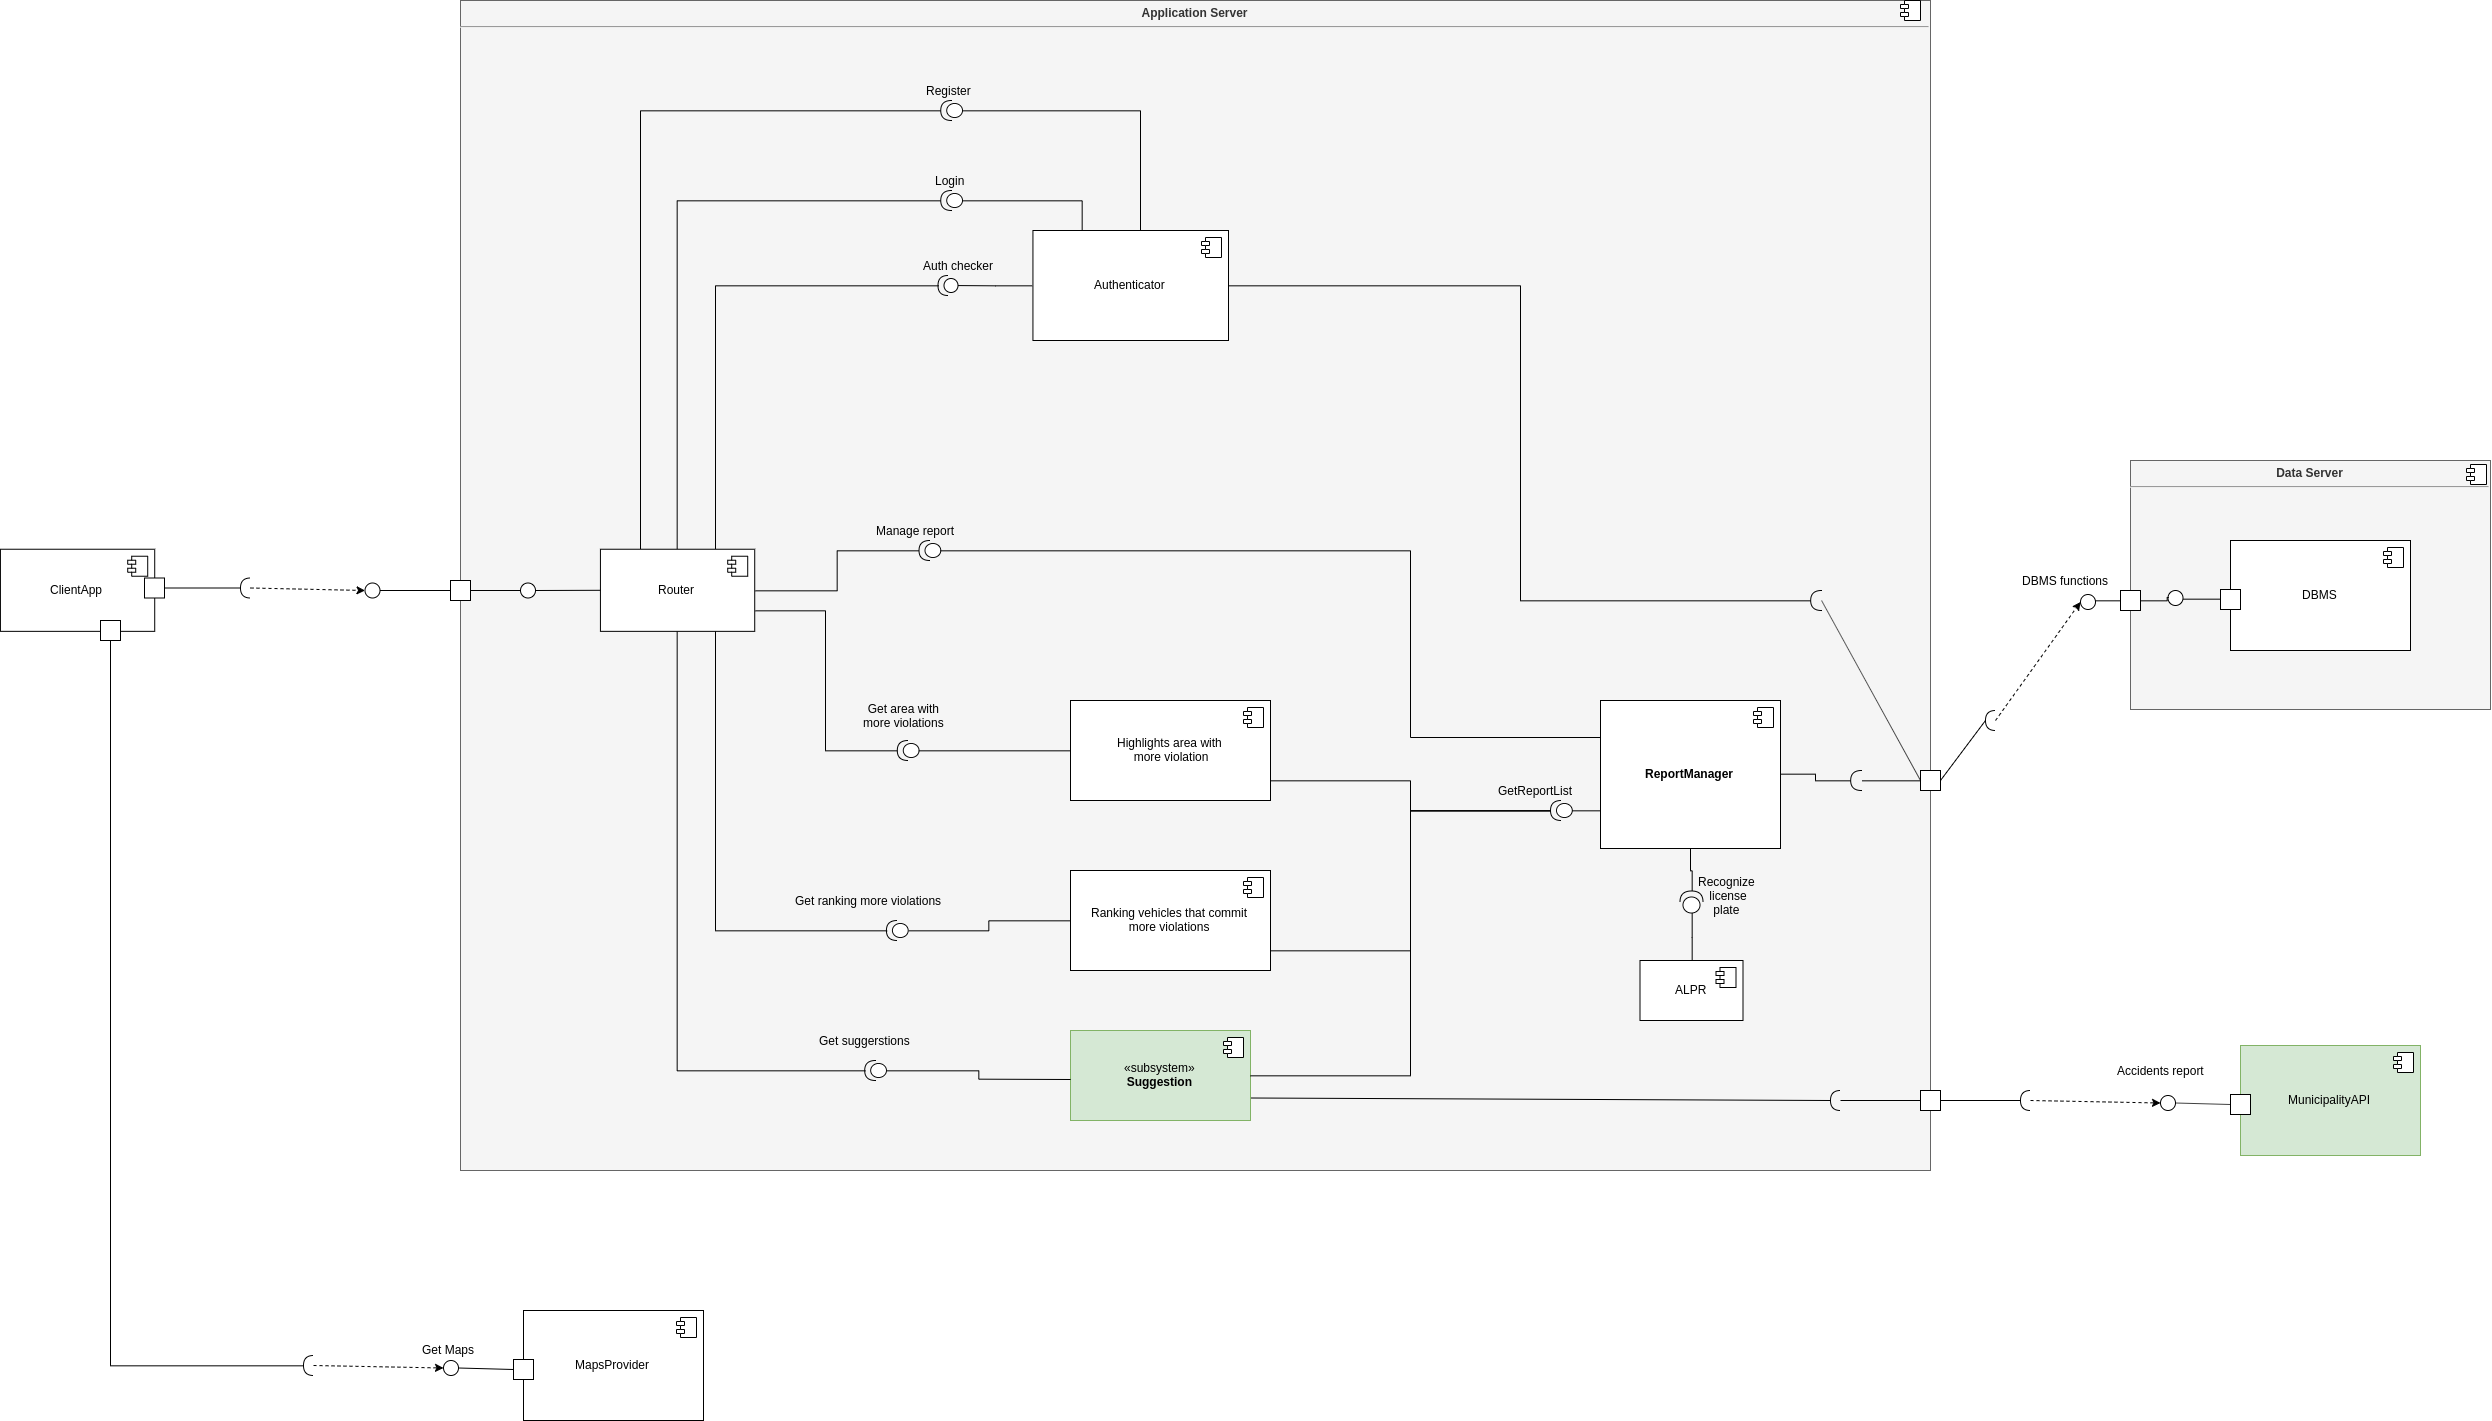
\includegraphics[width=1.0\textwidth]{images/components-diagram.png}
	\caption{Component diagram}
	\label{fig:component-diagram}
\end{figure}

Here are described more in detail all the components and interfaces that
the application server uses to offer its functionalities.
\begin{itemize}
	\item \textbf{Router}: Manages all the request coming from the clients, forwarding them in the appropriate component for the specific request. 
	It also interacts with the \textit{Authenticator component} to check if a request comes from an authenticated user and then denies or forwards the request according to the user permissions.
	\item \textbf{Authenticator}: Manages the sign up and login requests and checks if a request comes from an authenticated user.
	\item \textbf{ReportManager}: Manages all the requests inerent to reports (e.g. get list of report, send new report) and is responsible to check if the new reports are consistent. Also collects reports form the database to pass them to other components.
	\item \textbf{Area-Highlighter}: Elaborates the reports to find in which area more violations are committed.
	\item \textbf{RankingManager}: Elaborates the valid reports to create a ranking of the vehicles that committed more violations.
	\item \textbf{SuggestionSubsystem}: More in detail:
		\\
	\item \textbf{NotificationManager}: Manage all the subscriptions for notification made by the client's app when a traffic warden log in and send the notification to them when a new report is added.
	\item \textbf{ALPR}: Elaborates the picture of the violation to extract the license plate. This component is designed to be separate by the others so that if after deployment it will became overload it could be deployed on a different server.
\begin{figure}[ht]
\centering
	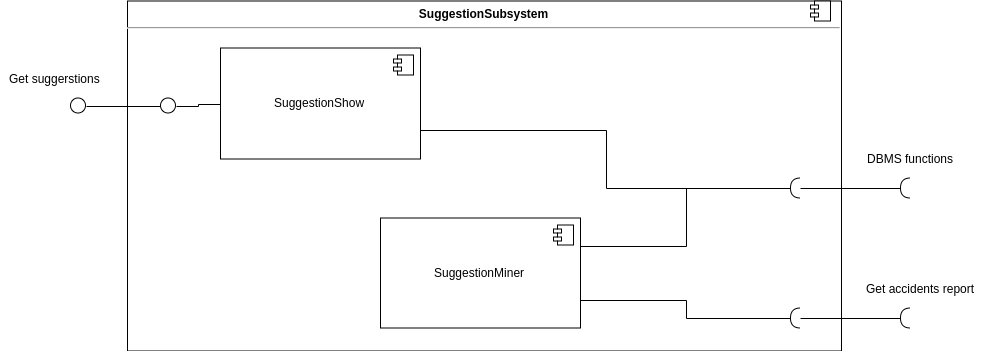
\includegraphics[width=1.0\textwidth]{images/SuggestionSubsystem-components-diagram.png}
	\caption{Component diagram suggestion subsystem}
	\label{fig:component-suggestion-subsystem}
\end{figure}
	\item \textbf{SuggestionDisplayer}: Sends the list of the suggestions
	\item \textbf{SuggestionMiner}: Gets data from Muncipality's servers and from Safestreets' database and elaborates the suggestions for possible interventions
\end{itemize}

\newpage

\subsection{Deployment view}
The following diagram models the physical deployment of artifacts (software components) on nodes (hardware components).
External services like the Map Provider are not included.
\begin{figure}[ht]
\centering
	\includegraphics[width=1.0\textwidth]{images/deployment_diagram.png}
	\caption{Deployment diagram}
	\label{fig:deployment-diagram}
\end{figure}

	
\begin{itemize}
	\item \textbf{Tier 1} Users can access the SafeStreets service using the mobile application available for Android and iOS devices or using the web app (compatible with any modern browser).
	\item \textbf{Tier 2} The same server machine (for budget reasons)  will contain all the components handling the business and the web logic. The application server handles all the requests coming from the users applications. The web server is just there to make possible to get the web app from the website. The web app will communicate directly with the application server using RESTful API.
	\item \textbf{Tier 3} The database machine will run MySQL server (a relational database management system). On this machine will be stored all the persistent data.
\end{itemize}

\newpage

\subsection{Runtime view}
 2.4 interactions seq diagrams, more details on diagrams used in RASD (in rasd no breakdown of components) (here we highlights of system respond to interaction from outside, which components? )
 \\ In this section are shown the sequence diagrams of some features. They are useful to clarify the
runtime behaviour of the components involved for each functionality.

\subsection{Component interfaces}
Details on method on interfaces previously indentified, consistency check ( labels messages used in runtimeview consistent with the interfaces of components)
\\
use tables ?
\subsection{Selected architectural styles and patterns}
list all design decisions (al least references to ...) explain how they're used , variants...

\subsection{Other design decisions}

\section{User interface design}

\section{Requirements traceability}

\section{Implementation, integration and test plan}

\section{Effort spent}
	\begin{center}
		{\bf Cazzola Federico \href{https://github.com/f-cazzola}{@f-cazzola} }
		\vspace{2mm}

			\begin{tabular}{p{1.3cm}|p{1.8cm}|p{6.7cm}}
				\hline
				\bf Date & \bf \makebox[1.8cm][c]{Hours} & \bf \makebox[6.7cm][c]{Description} \\
				23/11/19 & \makebox[1.8cm][c]{2} & \makebox[6.7cm][c]{Architectural design}\\
				24/11/19 & \makebox[1.8cm][c]{3} & \makebox[6.7cm][c]{Architectural design}\\
				29/11/19 & \makebox[1.8cm][c]{2} & \makebox[6.7cm][c]{Architectural design}\\
				30/11/19 & \makebox[1.8cm][c]{4} & \makebox[6.7cm][c]{Architectural design}\\
				\hline
				total    & \makebox[1.8cm][c]{11}
			\end{tabular}
	\end{center}
	\vspace{1cm}

	\begin{center}
		{\bf Dotti Francesco \href{https://github.com/dottif}{@dottif} }
		\vspace{2mm}

			\begin{tabular}{p{1.3cm}|p{1.8cm}|p{6.7cm}}
				\hline
				\bf Date & \bf \makebox[1.8cm][c]{Hours} & \bf \makebox[6.7cm][c]{Description} \\
				\hline
				15/11/19 & \makebox[1.8cm][c]{1} & \makebox[6.7cm][c]{Initial Structure}\\
				22/11/19 & \makebox[1.8cm][c]{1.5} & \makebox[6.7cm][c]{Introduction}\\
				23/11/19 & \makebox[1.8cm][c]{1.5} & \makebox[6.7cm][c]{Architectural design}\\
				29/11/19 & \makebox[1.8cm][c]{0.5} & \makebox[6.7cm][c]{Component view}\\
				30/11/19 & \makebox[1.8cm][c]{4} & \makebox[6.7cm][c]{Component and Deployment view}\\
				\hline
				total    & \makebox[1.8cm][c]{8.5}
			\end{tabular}
	\end{center}

\end{document}
